%\documentclass{article}
%\usepackage{graphicx,subfigure}
%\begin{document}

\begin{figure}[h]
  \centering
   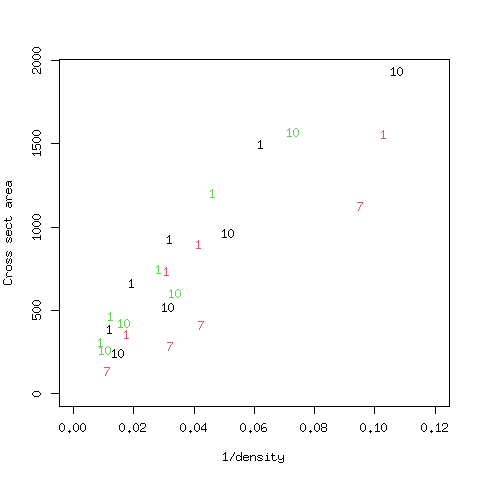
\includegraphics[width=0.9\textwidth]{DC1955/dc123.png}
  \caption{Plot of breed means for reciprocal of follicle density and fibre cross sectional area from Daly and Carter(1956)~\cite{daly:56}  all 3 experiments .  The black points are experiment 1, the red points are experiment 2, the green points are experiment 3.}
  \label{fig:dc123}
\end{figure}

%\end{document}

